\chapter{Object Reconstruction and Selection}

feature properties well suited to particle-flow (PF) reconstruction: a highly-segmented tracker, a fine-grained electromagnetic calorimeter, a hermetic hadron calorimeter, a strong magnetic field, and an excellent muon spectrometer.

For each collision, the comprehensive list of final-state particles identified and reconstructed by the algorithm provides a global event description that leads to unprecedented CMS performance for jet and hadronic $\tau$ decay reconstruction, missing transverse momentum determination, and electron and muon identification.

This approach also allows particles from pileup interactions to be identified and enables efficient pileup mitigation methods.


\begin{figure*}[htbp]
\centering
     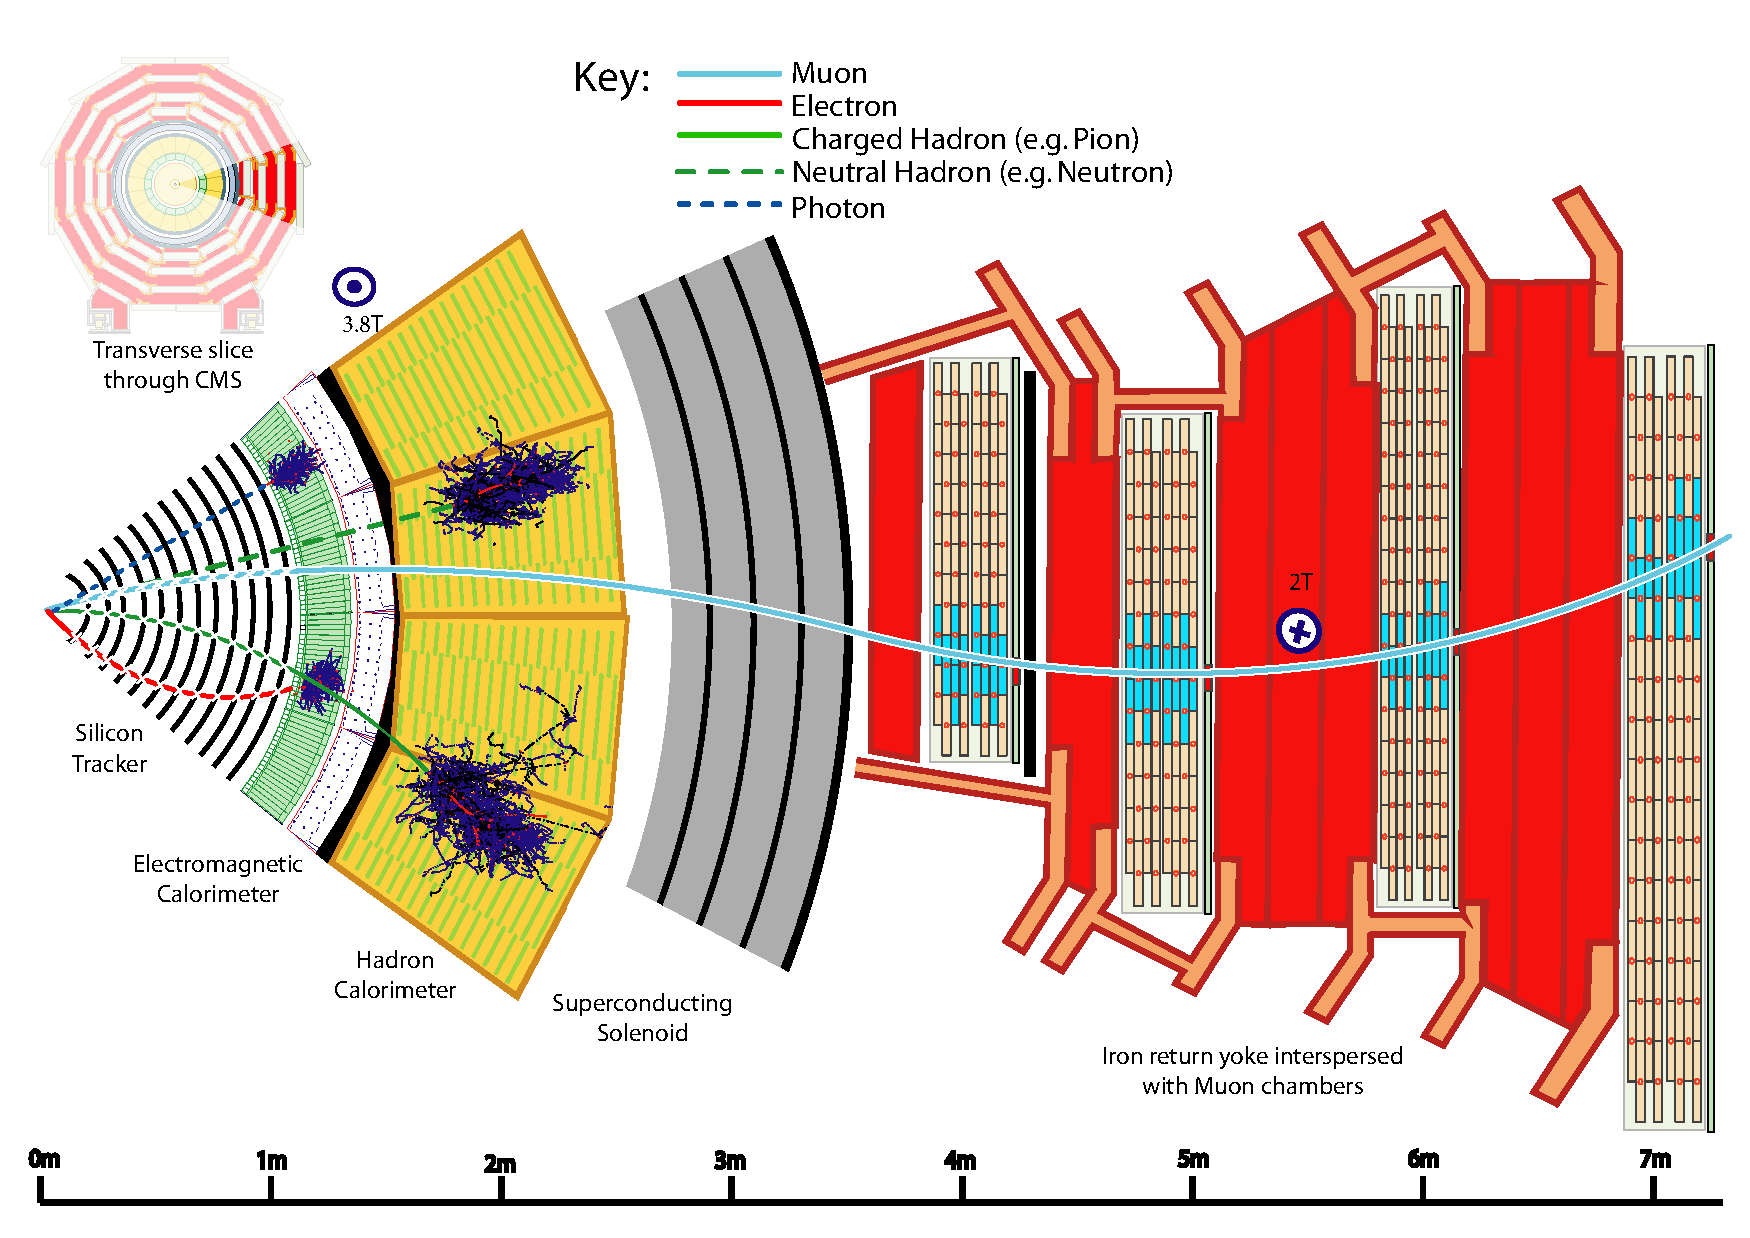
\includegraphics[width=1.0\textwidth]{object_reconstruction_and_selection/plots/cms_slice.pdf}
     \caption{
     }
     \label{fig:cms_slice}
\end{figure*}

A significantly improved event description can be achieved by correlating the basic elements from all detector layers (tracks and clusters) to identify each final-state particle, and by combining the corresponding measurements to reconstruct the particle properties on the basis of this identification. This holistic approach is called particle-flow (PF) reconstruction.

--- a large magnetic field, to separate the calorimeter energy deposits of charged and neutral
---articles in jets;
--- afine-grainedtracker,providingapureandefficientcharged-particletrajectoryreconstruction in jets with pT up to around 1 TeV, and therefore an excellent measurement of ∼65\% of the jet energy;
--- a highly-segmented ECAL, allowing energy deposits from particles in jets (charged hadrons, neutral hadrons, and photons) to be clearly separated from each other up to a jet pT of the order of 1 TeV. The resulting efficient photon identification, coupled to the high ECAL energy resolution, allows for an excellent measurement of another ∼25\% of the jet energy;
--- a hermetic HCAL with a coarse segmentation, still sufficient to separate charged and neutral hadron energy deposits in jets up to a jet pT of 200–300 GeV, allowing the remaining 10\% of the jet energy to be reconstructed, although with a modest resolution;
--- an excellent muon tracking system, delivering an efficient and pure muon identification, irrespective of the surrounding particles.




\section{Track and Primary Vertex Reconstruction}

measuring the momentum of energetic and isolated muons, at identifying energetic and isolated hadronic τ decays, and at tagging b quark jets. Tracking was therefore primarily targeting energetic particles and was limited to well- measured tracks.

A combinatorial track finder based on Kalman Filtering (KF) was used to reconstruct these tracks in three stages: initial seed generation with a few hits compatible with a charged-particle trajectory; trajectory building (or pattern recognition) to gather hits from all tracker layers along this charged-particle trajectory; and final fitting to determine the charged- particle properties: origin, transverse momentum, and direction.
To be kept for further analysis, the tracks had to be seeded with two hits in consecutive layers in the pixel detector, and were required to be reconstructed with at least eight hits in total and with at most one missing hit along the way.

\begin{figure*}[htbp]
\centering
     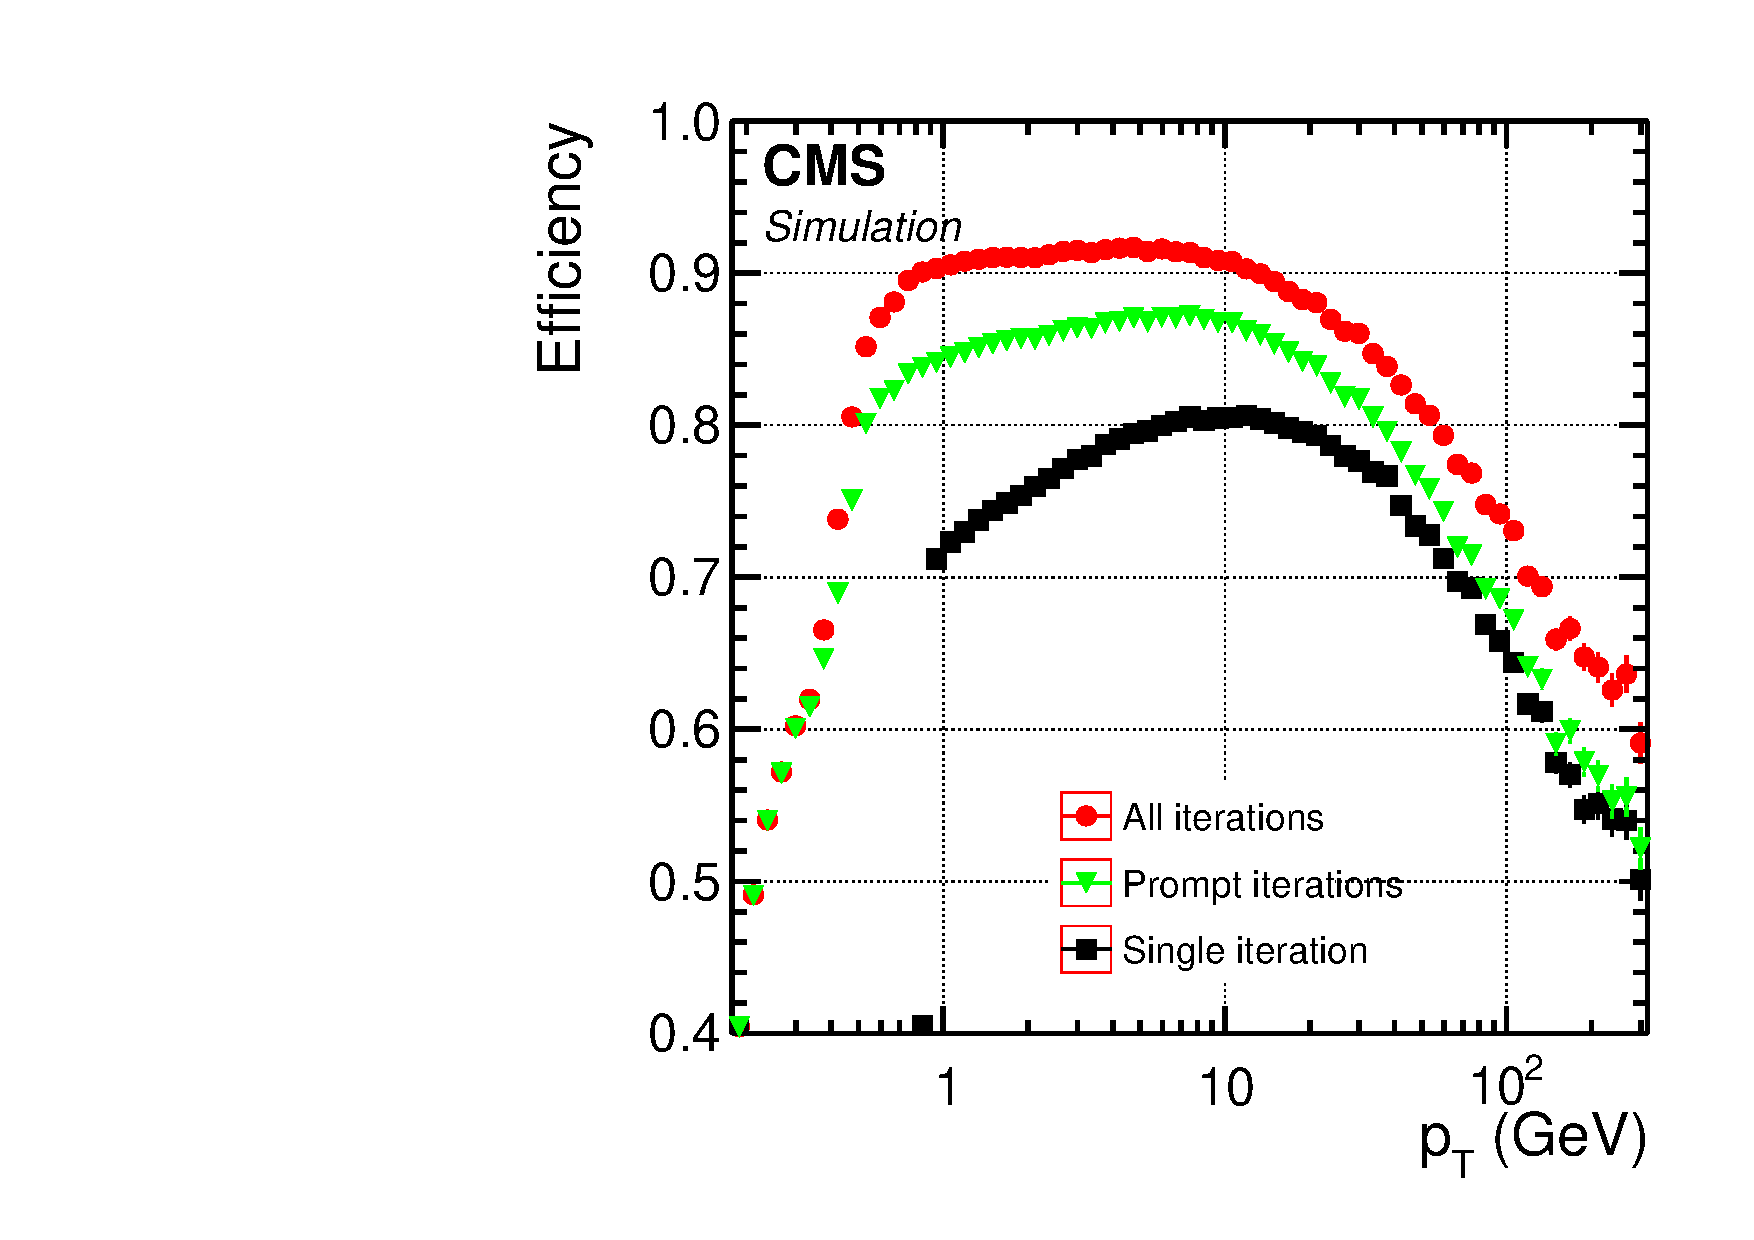
\includegraphics[width=0.45\textwidth]{object_reconstruction_and_selection/plots/pf_track_eff.pdf}
     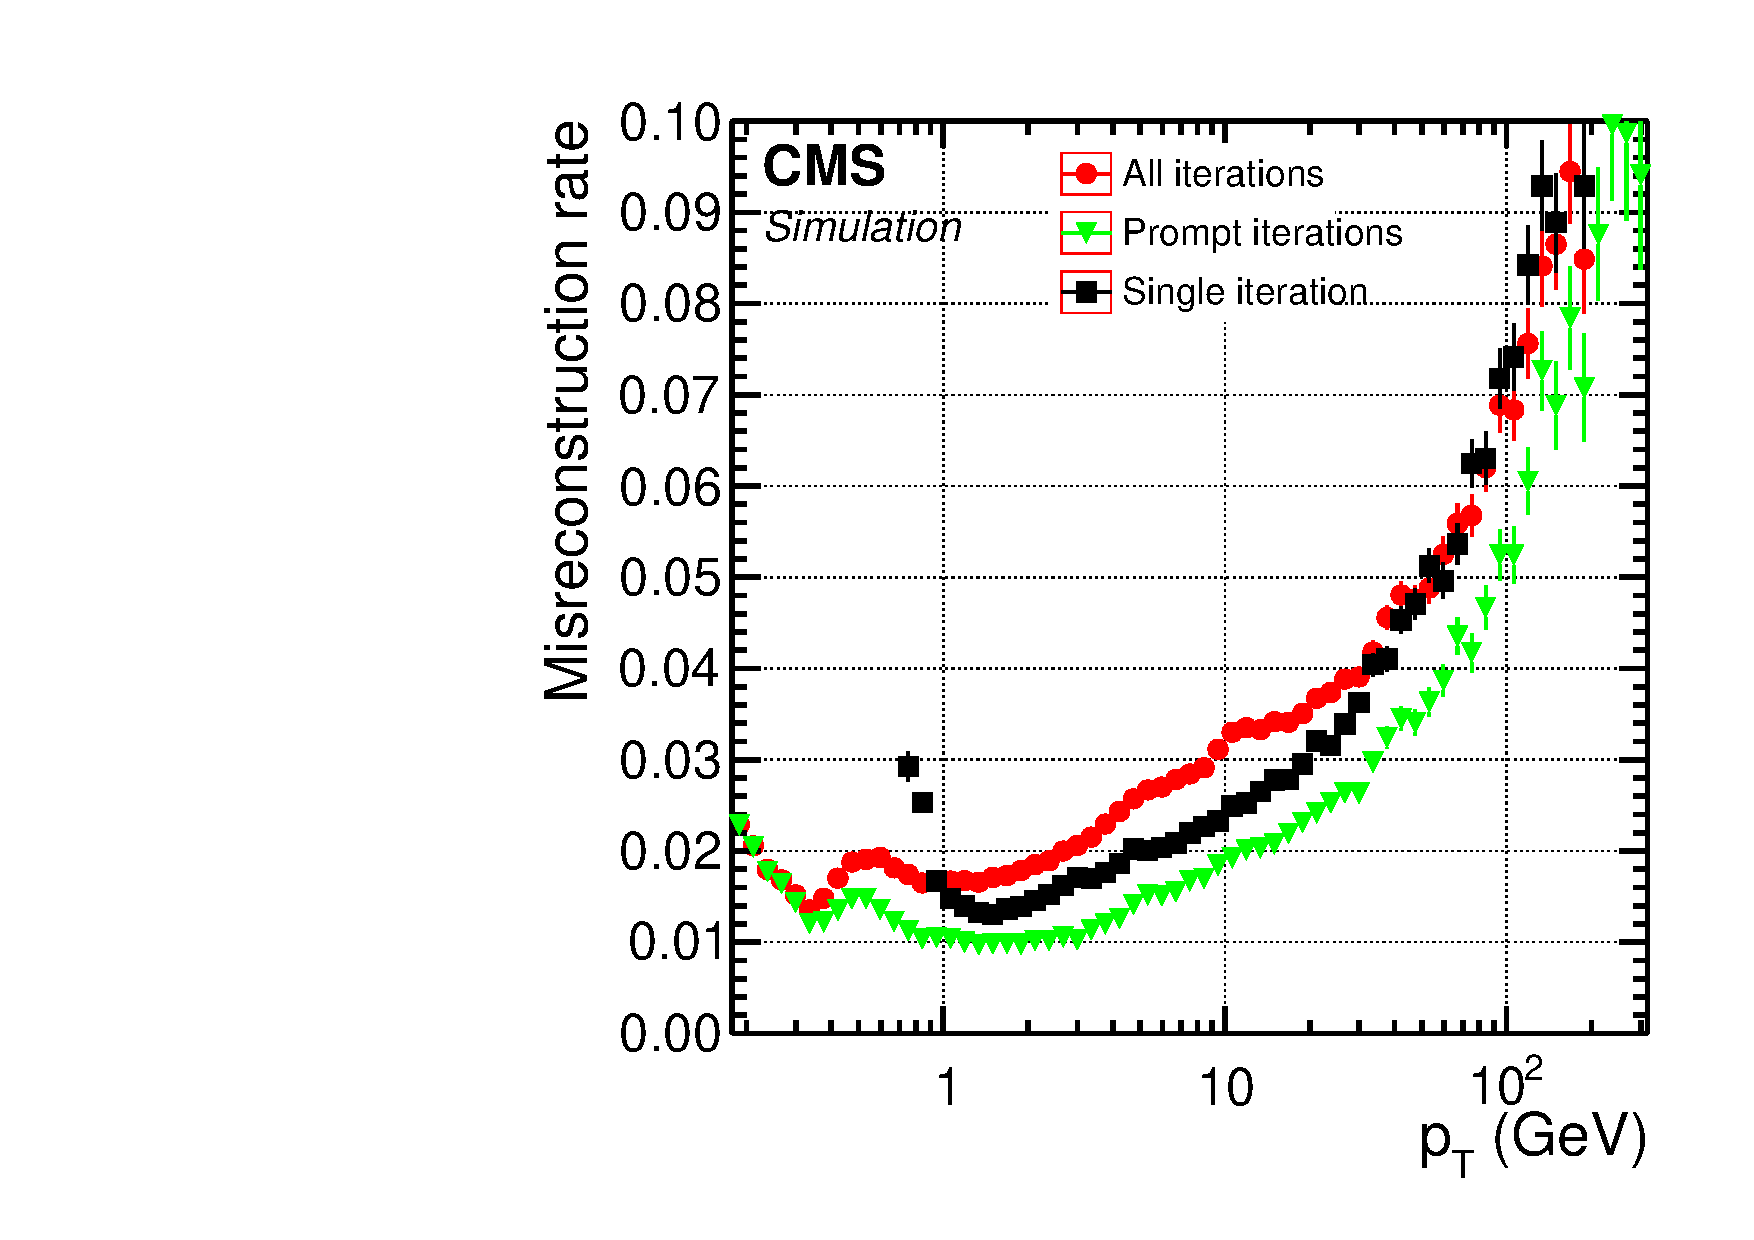
\includegraphics[width=0.45\textwidth]{object_reconstruction_and_selection/plots/pf_track_misId.pdf}
     \caption{
Efficiency (left) and misreconstruction rate (right) of the global combinatorial track finder (black squares); 
and of the iterative tracking method (green triangles: prompt iterations based on seeds with at least one 
hit in the pixel detector; red circles: all iterations, including those with displaced seeds), as a function 
of the track $\pt$, for charged hadrons in multijet events without pileup interactions. Only tracks with 
$\abs\eta < 2.5$ are considered in the efficiency and misreconstruction rate determination. The efficiency 
is displayed for tracks originating from within 3.5 cm of the beam axis and $\pm$30 cm of the nominal 
centre of CMS along the beam axis.
     }
     \label{fig:cms_slice}
\end{figure*}

stringent track quality criteria are instrumental in keeping the misreconstructed track rate at the level of a few per cent, but limit the reconstruction efficiency to only 70–80\% for charged pions with pT above 1 GeV, compared to 99\% for isolated muons.
The probability for a hadron to interact within the tracker material, before reaching the eight-hits threshold 
-- causing the track to be missed -- ranges between 10 and 30\%. The tracking efficiency is further 
reduced for $\pt$ values above 10GeV: these high-pT particles are found mostly in collimated jets, in 
which the tracking efficiency is limited by the silicon detector pitch, i.e. by the capacity to 
disentangle hits from overlapping particles.

Iterative Tracking
To increase the tracking efficiency while keeping the misreconstructed track rate at a similar level, the combinatorial track finder was applied in several successive iterations, each with moderate efficiency but with as high a purity as possible. At each step, the reduction of the misreconstruction rate is accomplished with quality criteria on the track seeds, on the track fit $\chi^2$, and on the track compatibility with originating from one of the reconstructed primary vertices, adapted to the track $\pt$, $\abs\eta$, and number of hits nhits. In practice, no quality criteria are applied to tracks reconstructed with at least eight hits, as the misreconstruction rate is already small enough for these tracks. The hits associated with the selected tracks are masked in order to reduce the probability of random hit-to-seed association in the next iteration. The remaining hits may thus be used in the next iteration to form new seeds and tracks with relaxed quality criteria, increasing in turn the total tracking efficiency without degrading the purity. The same operation is repeated several times with progressively more complex and time-consuming seeding, filtering, and tracking algorithms.
With an overall efficiency of $\sim 80\%$, the fractions of hits masked for the next iterations amount to 40\% (20\%) in the pixel (strip) detector.
Despite the significant improvement, the tracking efficiency at high pT remains limited. The consequences for jet energy and angular resolutions are minute, as the calorimeter resolutions are already excellent at these energies. The significant increase of the misreconstructed track rate at high pT is dealt with when the information from the calorimeters and the muon system becomes available


Electron Tracking
for electrons with small pT, whose tracks are significantly bent by the magnetic field, the radiated energy is spread over such an extended region that the supercluster cannot include all deposits.

When energetic photons are radiated, the pattern recognition may be unable to accommodate the change in electron momentum, causing the track to be reconstructed with a small number of hits. A preselection based on the number of hits and the fit $\chi^2$ is therefore applied and the selected tracks are fit again with a Gaussian-sum filter (GSF)

The GSF fitting is more adapted to electrons than the KF used in the iterative tracking, as it allows for sudden and substantial energy losses along the trajectory.

The tracker-based seeding is also effective at selecting electrons and positrons from conversions in the tracker material, for both prompt and bremsstrahlung photons. The recovery of the converted photons of the latter category and their association to their parent electrons is instrumental in minimizing energy double counting in the course of the PF reconstruction.


Muon Tracks
A high purity is granted by the upstream calorimeters, meant to absorb other particles (except neutrinos). The inner tracker provides a precise measurement of the momentum of these muons.

standalone muon. Hits within each DT or CSC detector are clustered to form track segments, used as seeds for the pattern recognition in the muon spectrometer, to gather all DT, CSC, and RPC hits along the muon trajectory.

global muon. Each standalone-muon track is matched to a track in the inner tracker (hereafter referred to as an inner track) if the parameters of the two tracks propagated onto a common surface are compatible. The hits from the inner track and from the standalone-muon track are combined and fit to form a global-muon track.

tracker muon. Each inner track with pT larger than 0.5 GeV and a total momentum p in excess of 2.5 GeV is extrapolated to the muon system. If at least one muon segment matches the extrapolated track, the inner track qualifies as a tracker muon track.

about 99\% of the muons produced within the geometrical acceptance of the muon system are reconstructed either as a global muon or a tracker muon and very often as both.


Calorimeter Clusters
The purpose of the clustering algorithm in the calorimeters is fourfold: (i) detect and measure the energy and direction of stable neutral particles such as photons and neutral hadrons; (ii) separate these neutral particles from charged hadron energy deposits; (iii) reconstruct and identify electrons and all accompanying bremsstrahlung photons; and (iv) help the energy measurement of charged hadrons for which the track parameters were not determined accurately, which is the case for low-quality and high-pT tracks.

aims of a high detection efficiency even for low-energy particles and of separating close energy deposits, as illustrated in figure 2. The clustering is performed separately in each subdetector: ECAL barrel and endcaps, HCAL barrel and endcaps, and the two preshower layers.

cluster seeds are identified as cells with an energy larger than a given seed threshold, and larger than the energy of the neighbouring cells

topological clusters are grown from the seeds by aggregating cells with at least a corner in common with a cell already in the cluster and with an energy in excess of a cell threshold set to twice the noise level.

The Gaussian-mixture model postulates that the energy deposits in the M individual cells of the 
topological cluster arise from N Gaussian energy deposits where N is the number of seeds.


ECAL
A residual energy calibration, required to account for the effects of these thresholds, is determined from simulated single photons. This generic calibration is applied to all ECAL clusters prior to the hadron cluster calibration discussed in the next section, and to the particle identification step described following.

HCAL
the calorimeter response depends on the fraction of the shower energy deposited in the ECAL, and is not linear with energy. The ECAL and HCAL cluster energies therefore need to be substantially recalibrated to get an estimate of the true hadron energy.

simulated single neutral hadrons (specifically, KL0) is used to determine the calibration coefficients


\begin{figure*}[htbp]
\centering
     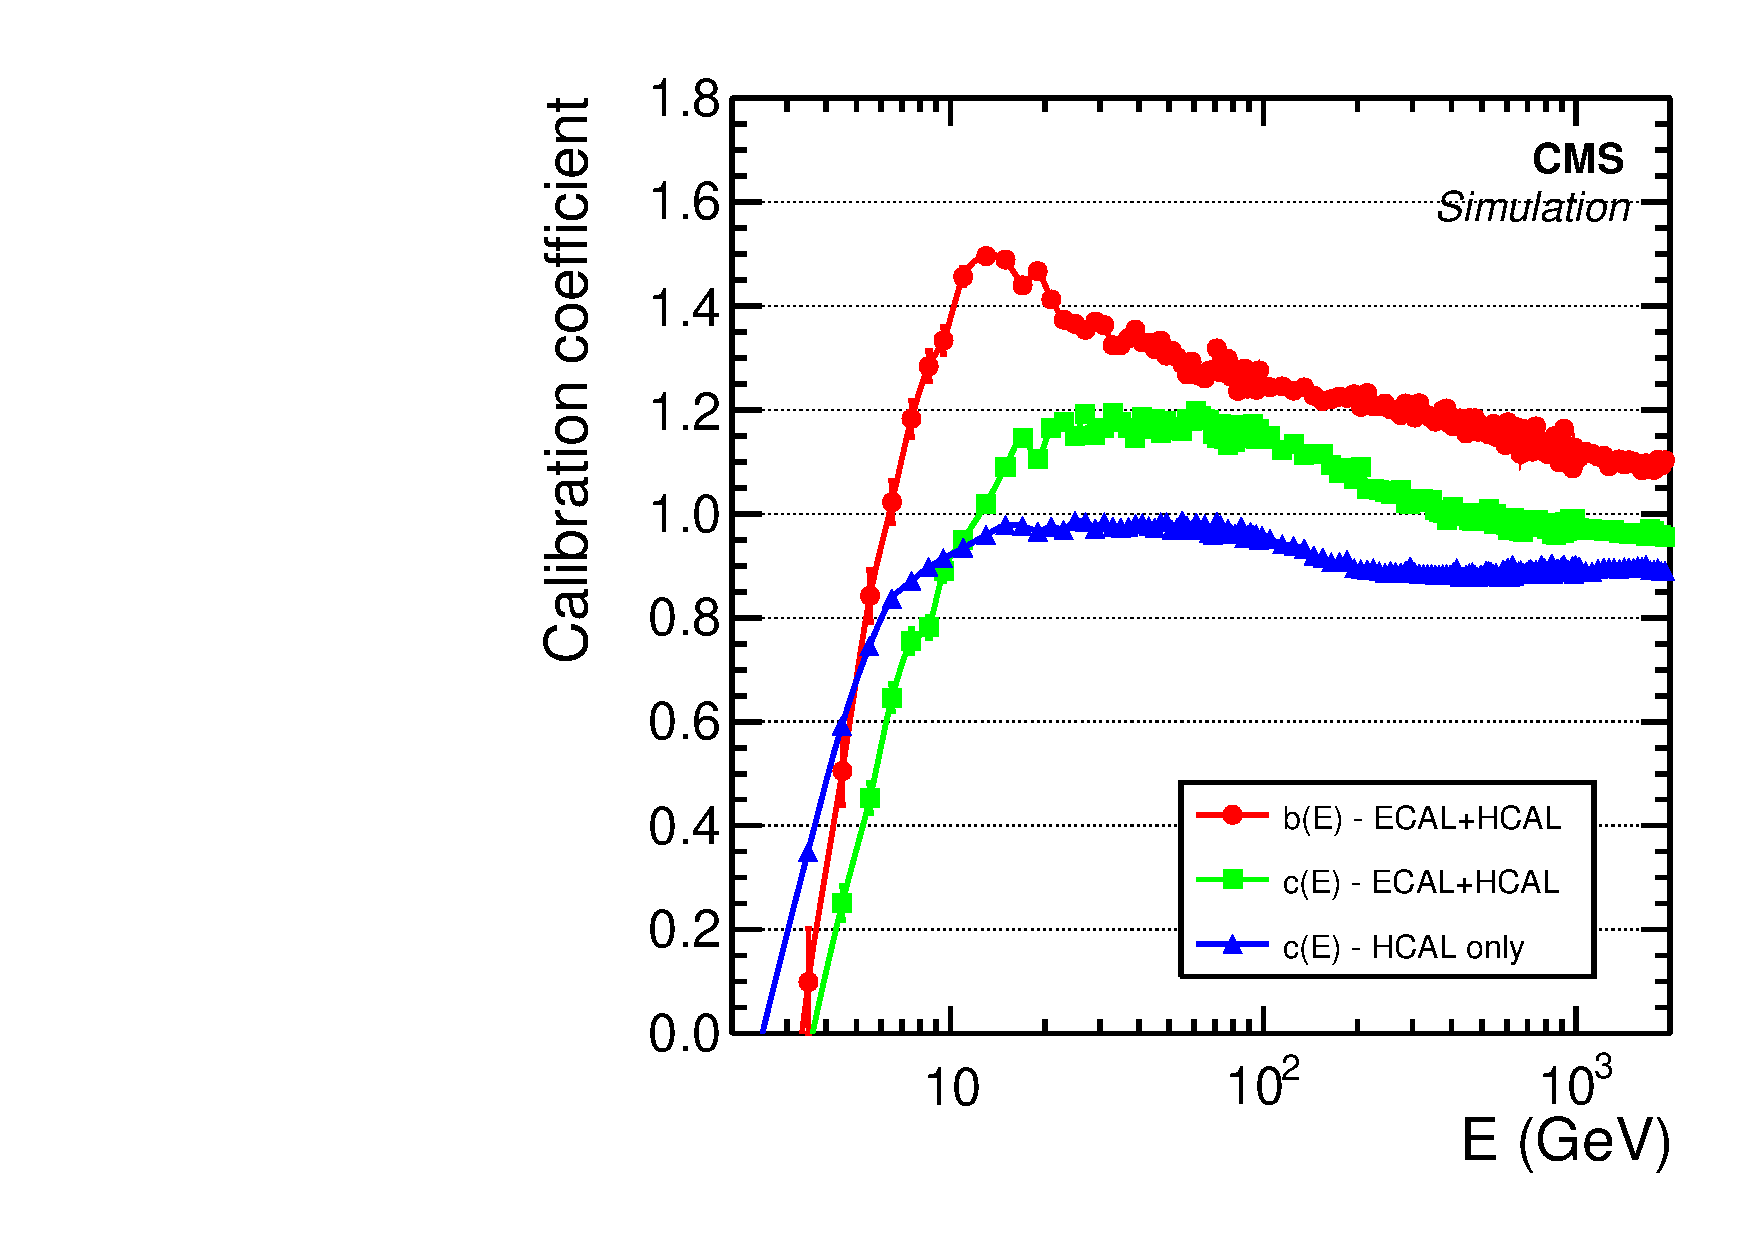
\includegraphics[width=0.45\textwidth]{object_reconstruction_and_selection/plots/calo_calibrations.pdf}
     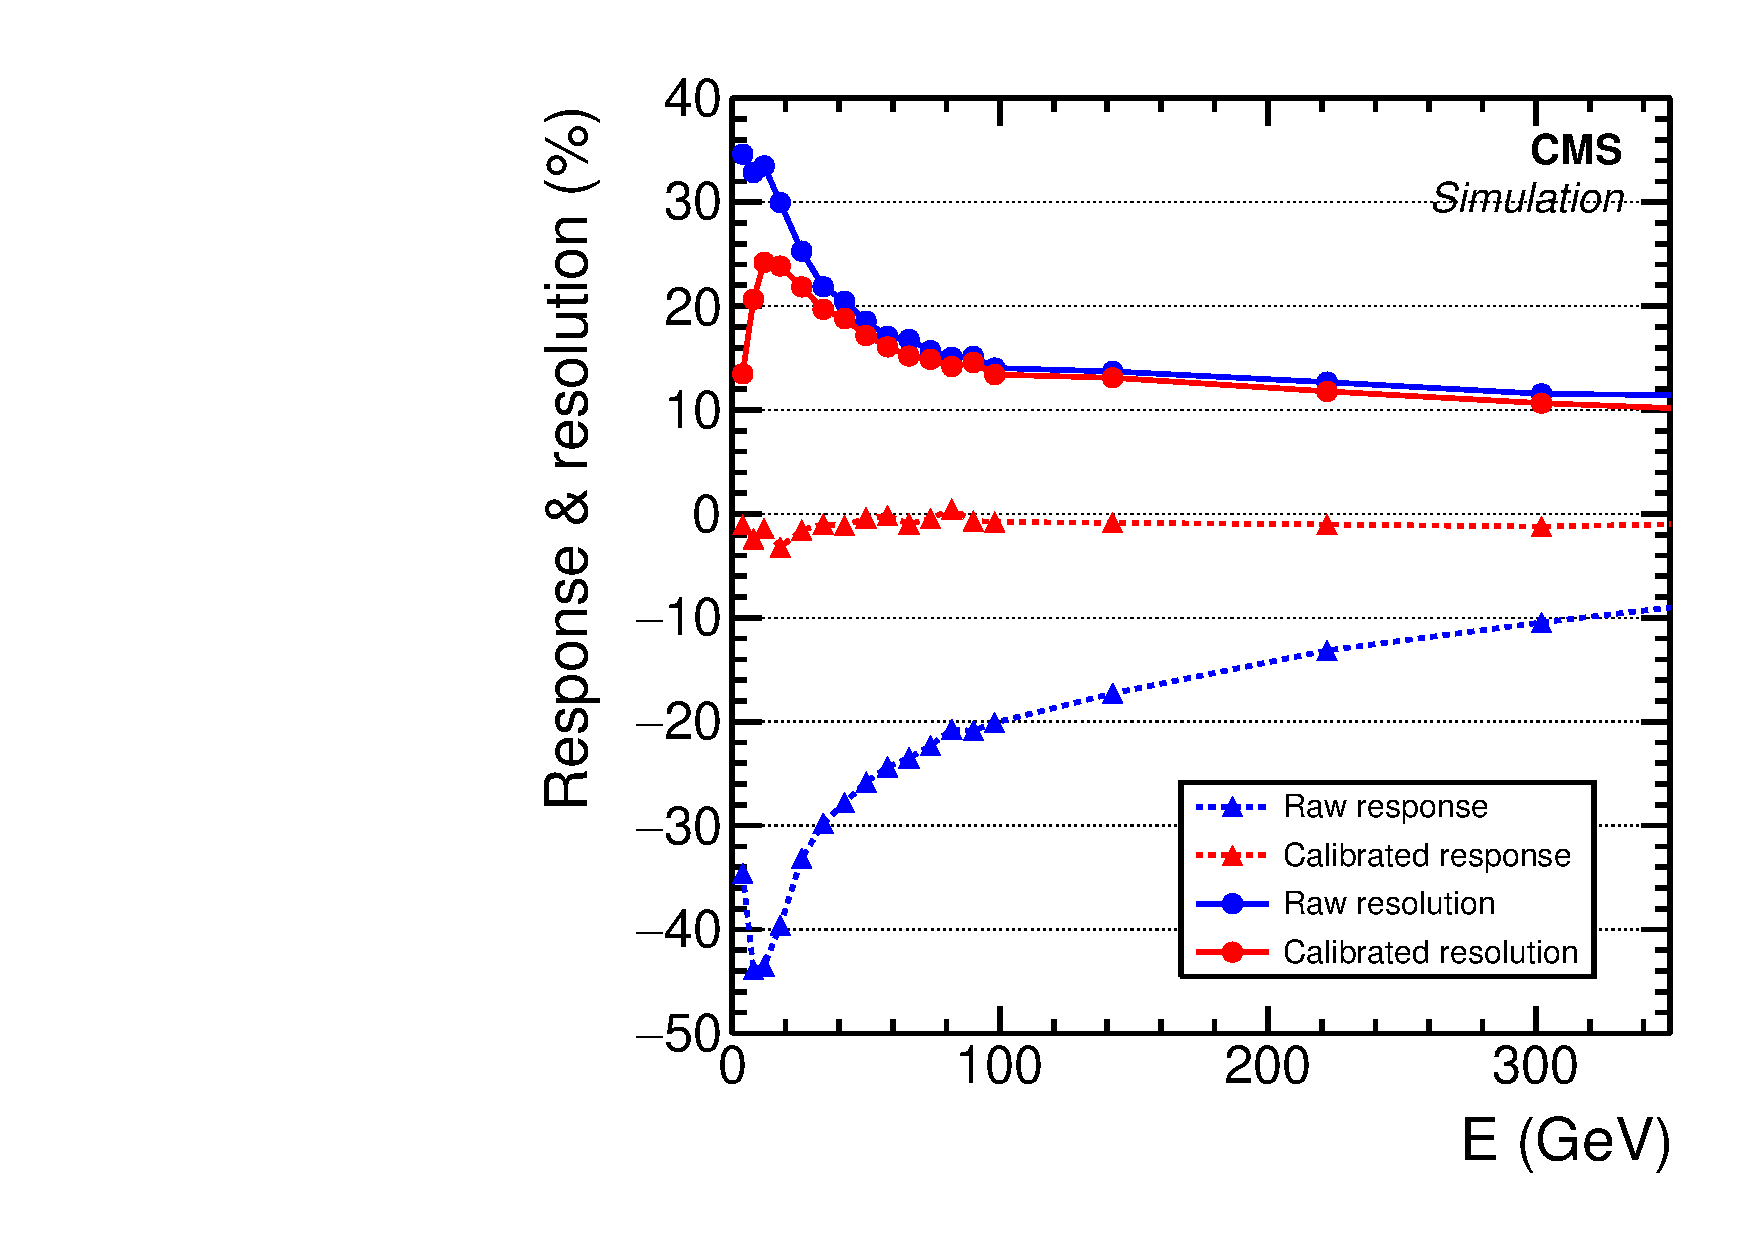
\includegraphics[width=0.45\textwidth]{object_reconstruction_and_selection/plots/calo_response_and_res.pdf}
     \caption{
Left: Calibration coefficients obtained from single hadrons in the barrel as a function of their true energy E, for hadrons depositing energy only in the HCAL (blue triangles), and for hadrons depositing energy in both the ECAL and HCAL, for the ECAL (red circles) and for the HCAL (green squares) clusters. Right: Relative raw (blue) and calibrated (red) energy response (dashed curves and triangles) and resolution (full curves and circles) for single hadrons in the barrel, as a function of their true energy E. Here the raw (calibrated) response and resolution are obtained by a Gaussian fit to the distribution of the relative difference between the raw (calibrated) calorimetric energy and the true hadron energy.
     }
     \label{fig:cms_slice}
\end{figure*}

it is worth stressing at this point that this calibration affects only 10\% of the measured event energy. The latter is therefore expected to be modified, on average, by
only a few per cent by the calibration procedure.


Linking
A given particle is, in general, expected to give rise to several PF elements in the various CMS subdetectors. The reconstruction of a particle therefore first proceeds with a link algorithm that connects the PF elements from different subdetectors.

The link algorithm then produces PF blocks of elements associated either by a direct link or by an indirect link through common elements.

a link between a track in the central tracker and a calorimeter cluster is established as follows. The track is first extrapolated from its last measured hit in the tracker to — within the corresponding angular acceptance — the two layers of the preshower, the ECAL at a depth corresponding to the expected maximum of a typical longitudinal electron shower profile, and the HCAL at a depth corresponding to one interaction length.

The link distance is defined as the distance between the extrapolated track position and the cluster position in the \etaphi plane.

In case several HCAL clusters are linked to the same track, or if several tracks are linked to the same ECAL cluster, only the link with the smallest distance is kept.

Calorimeter cluster-to-cluster links are sought between HCAL clusters and ECAL clusters, and between ECAL clusters and preshower clusters in the preshower acceptance. A link is established when the cluster position in the more granular calorimeter (preshower or ECAL) is within the cluster envelope in the less granular calorimeter (ECAL or HCAL).

Charged-particle tracks may also be linked together through a common secondary vertex, for nuclear-interaction reconstruction

Finally, a link between a track in the central tracker and information in the muon detector is established to form global and tracker muons.

\section{Particle Flow Reconstruction}
\subsection{PF Candidates}
\subsubsection{Muons}

Isolated global muons are first selected by considering additional inner tracks and calorimeter 
energy deposits with a distance $\Delta$ R to the muon direction in the \etaphi plane smaller than 0.3. 
The sum of the pT of the tracks and of the ET of the deposits is required not to exceed 10\% of the 
muon $\pt$. This isolation criterion alone is sufficient to adequately reject hadrons that would be 
misidentified as muons, hence no further selection is applied to these muon candidates.

For nonisolated global muons, the tight-muon selection is applied. In addition, it is required either that at least three matching track segments be found in the muon detectors, or that the calorimeter deposits associated with the track be compatible with the muon hypothesis. This selection removes the majority of high-pT hadrons misidentified as muons because of punch- through, as well as accidental associations of tracker and standalone muon tracks.

The muon momentum is chosen to be that of the inner track if its pT is smaller than 200 GeV. Above this value, the momentum is chosen according to the smallest $\chi^2$ probability from the different track fits: tracker only, tracker and first muon detector plane, global, and global without the muon detector planes featuring a high occupancy

The PF elements that make up these identified muons are masked against further processing in the corresponding PF block

\subsubsection{Electrons and Prompt Photons}

Electron reconstruction is based on combined information from the inner tracker and the calori- meters. Due to the large amount of material in the tracker, electrons often emit bremsstrahlung photons and photons often convert to e+e− pairs

Isolated photon reconstruction is therefore conducted together with electron reconstruction. In a given PF block, an electron candidate is seeded from a GSF track, as described in section 3.2, provided that the corresponding ECAL cluster is not linked to three or more additional tracks. A photon candidate is seeded from an ECAL supercluster with ET larger than 10 GeV, with no link to a GSF track.

sum of the energies measured in the HCAL cells with a distance to the supercluster position smaller than 0.15 in the \etaphi plane must not exceed 10\% of the supercluster energy.

The final energy assignment for electrons is obtained from a combination of the corrected ECAL energy with the momentum of the GSF track and the electron direction is chosen to be that of the GSF track

Electron candidates must satisfy additional identification criteria. Specifically, up to fourteen variables — including the amount of energy radiated off the GSF track, the distance between the GSF track extrapolation to the ECAL entrance and the position of the ECAL seeding cluster, the ratio between the energies gathered in HCAL and ECAL by the track-cluster association process, and the KF and GSF track $\chi^2$ and numbers of hits — are combined in BDTs trained separately in the ECAL barrel and endcaps acceptance, and for isolated and nonisolated electrons.

Photon candidates are retained if they are isolated from other tracks and calorimeter clusters in the event, and if the ECAL cell energy distribution and the ratio between the HCAL and ECAL energies are compatible with those expected from a photon shower.



\subsubsection{Charged and Neutral Hadrons}

Once muons, electrons, and isolated photons are identified and removed from the PF blocks, the remaining particles to be identified are hadrons from jet fragmentation and hadronization. These particles may be detected as charged hadrons (π±, K±, or protons), neutral hadrons (e.g. KL0 or neutrons), nonisolated photons (e.g. from π0 decays), and more rarely additional muons (e.g. from early decays of charged hadrons).

The ECAL and HCAL clusters not linked to any track give rise to photons and neutral hadrons. Within the tracker acceptance (|η| < 2.5), all these ECAL clusters are turned into photons and all these HCAL clusters are turned into neutral hadrons. The precedence given in the ECAL to photons over neutral hadrons is justified by the observation that, in hadronic jets, 25\% of the jet energy is carried by photons, while neutral hadrons leave only 3% of the jet energy in the ECAL.

\subsection{Jets}

If the calibrated calorimetric energy is compatible with the sum of the track momenta, no neutral particle is identified.



\subsection{Taus}
\subsection{Missing Transverse Energy}

raw missing transverse momentum vector is defined in such a way as to balance the vectorial sum of the transverse momenta of all particles

\begin{equation}
\vec{p}^{\text{miss}}_{\text{T,PF}}(\text{raw}) = - \sum^{N_{\text{particles}}}_{i=1} \vec{p}_{\text{T},i}
\end{equation}

\pagebreak
\section{Object Identification and Selection}
\subsection{Muons}
\subsection{Electrons}
\subsection{Taus}
\subsection{b-jet ID and Secondary Vertex}





The reconstruction of observed and simulated events relies on the particle-flow (PF) algorithm~\cite{Sirunyan:2017ulk},
which combines the information from the CMS subdetectors to identify
and reconstruct the particles emerging from $\Pp\Pp$ collisions:
charged hadrons, neutral hadrons, photons, muons, and electrons.
Combinations of these PF objects are used to reconstruct
higher-level objects such as jets, $\tauh$ candidates, or
missing transverse energy.
The reconstructed vertex with the largest value of summed physics-object $\pt^2$ is taken to be the primary $\Pp\Pp$ interaction vertex. The physics objects are the objects constructed by a jet finding algorithm~\cite{Cacciari:2008gp,Cacciari:2011ma} applied to all charged tracks associated with the vertex, including tracks from lepton candidates, and the corresponding associated missing transverse energy.

Muons are identified with requirements on the quality of
the track reconstruction and on the number of measurements in the
tracker and the muon systems~\cite{Chatrchyan:2012xi}.
Electrons are identified with a multivariate discriminant
combining several quantities describing the track quality,
the shape of the energy deposits in the ECAL,
and the compatibility of the measurements from the tracker and the
ECAL~\cite{Khachatryan:2015hwa}.
To reject non-prompt or misidentified leptons, a relative lepton isolation is defined as:
\begin{equation}
I^{\ell} \equiv \frac{\sum_{charged}  \PT + \max\left( 0, \sum_{neutral}  \PT
                                         - \frac{1}{2} \sum_{charged, PU} \PT  \right )}{\PT^{\ell}}.
\label{eq:reconstruction_isolation}
\end{equation}
In this expression, $\sum_charged  \PT$ is the scalar sum of the
transverse energy of the charged particles originating from
the primary vertex and located in a cone of size
$\Delta R = \sqrt{\smash[b]{(\Delta \eta)^2 + (\Delta \phi)^2}} = 0.4$\,(0.3)
centered on the muon (electron) direction. The sum
$\sum_{neutral}  \PT$  represents
a similar quantity for neutral particles.
The contribution of photons and neutral hadrons originating from pileup vertices is estimated from the scalar sum of the transverse
energy of charged hadrons in the cone originating from pileup vertices,
$\sum_{charged, PU} \PT$. This sum is multiplied by a factor of
$1/2$, which corresponds approximately to the ratio of neutral to charged
hadron production in the hadronization process
of inelastic $\Pp\Pp$ collisions, as estimated from simulation.
The expression $\PT^{\ell}$ stands for the $\pt$ of the lepton. Isolation requirements used in this analysis, based on $I^{\ell}$, are listed in Table~\ref{tab:inclusive_selection}.

Jets are reconstructed with an anti-\kt clustering algorithm implemented
in the \FASTJET library~\cite{Cacciari:2011ma, Cacciari:fastjet2}.
It is based on the clustering of neutral and charged PF candidates within a distance parameter of 0.4. Charged PF candidates
not associated with the primary vertex of the interaction
are not considered when building jets. An offset correction is applied to jet energies to take into account the contribution from additional $\Pp\Pp$ interactions within the same or nearby bunch crossings. The energy of a jet is calibrated based on simulation and
data through correction factors~\cite{CMS-JME-10-011}.
In this analysis, jets are required to
have $\pt$ greater than 30\GeV and $\abs{\eta}$ less than 4.7, and
are separated from the selected leptons by a $\Delta R$ of at least 0.5.
The combined secondary vertex (CSV) algorithm is used to identify jets that are likely to originate from a b quark (``b jets"). The algorithm exploits the track-based lifetime information together with the secondary vertices associated with the jet to provide a likelihood ratio discriminator for the b jet identification. A set of $\pt$-dependent correction
factors are applied to simulated events to account for differences in the b tagging efficiency
between data and simulation. The working point chosen in this analysis gives an efficiency for real b jets of about 70\%, and for about 1\% of light flavor or quark jets being misidentified.

Hadronically decaying $\Pgt$ leptons
are reconstructed with the hadron-plus-strips (HPS)
algorithm~\cite{Khachatryan:2015dfa, CMS-PAS-TAU-16-002}, which is
seeded with anti-\kt jets.
The HPS algorithm reconstructs $\tauh$ candidates on the basis of the
number of tracks and of the number of ECAL strips in the $\eta$-$\phi$ plane with energy deposits, in the 1-prong,
1-prong + $\PGpz$(s), and 3-prong decay modes. A
multivariate (MVA) discriminator~\cite{Hocker:2007ht}, including isolation
and lifetime information, is used to reduce the rate for  quark- and gluon-initiated jets
to be identified as $\tauh$ candidates. The working point used in this analysis
has an efficiency of about 60\% for genuine $\tauh$,
with about 1\% misidentification rate for quark- and gluon-initiated jets, for a $\pt$ range typical of $\tauh$ originating from a $\PZ$ boson.
Electrons and muons misidentified as $\tauh$ candidates are suppressed using dedicated criteria
based on the consistency between the measurements in the tracker, the calorimeters, and the muon detectors~\cite{Khachatryan:2015dfa, CMS-PAS-TAU-16-002}.
The working points of these discriminators depend on the
decay channel studied.
The $\tauh$ energy scale in simulation is corrected per decay mode, on the basis of a measurement in $\PZ\to\Pgt\Pgt$ events. The rate and the
energy scale of electrons and muons misidentified as $\tauh$ candidates are also corrected in simulation, on the basis of a tag-and-probe measurement~\cite{CMS:2011aa} in $\PZ\to\ell\ell$ events.

All particles reconstructed in the event are used to determine the missing transverse energy,
\etvecmiss. The missing transverse momentum is defined as the negative vectorial sum of the transverse energy of
all PF candidates~\cite{Khachatryan:2014gga}. It is adjusted for the effect of jet energy corrections.
Corrections to the $\etvecmiss$ are applied to reduce the mismodeling of the simulated
$\PZ$+jets, $\PW$+jets and Higgs boson samples.
The corrections are applied to the simulated events on the basis of the vectorial difference
of the measured missing transverse energy and total transverse energy of neutrinos
originating from the decay of the $\PZ$, $\PW$, or Higgs boson. Their average effect is the reduction of the $\etvecmiss$ obtained from simulation by a few \GeV.

The visible mass of the $\Pgt\Pgt$ system, $\mvis$, can be used to separate
the $\PH\to \Pgt \Pgt$ signal events
from the large contribution of irreducible $\PZ \to \Pgt \Pgt$ events.
However, the neutrinos from the $\Pgt$ lepton decays carry a large fraction of
the $\Pgt$ lepton energy and reduce the discriminating power of this variable.
The \textsc{svfit} algorithm combines the \etvecmiss with the four-vectors of both $\Pgt$ candidates
to calculate a more accurate estimate of the mass of the parent boson, denoted as $\mtt$. The resolution of $\mtt$ is between 15 and 20\% depending on the $\Pgt\Pgt$ final state.
A detailed description of the algorithm can be found
in Ref.~\cite{Bianchini:2014vza}. Both variables are used in the analysis, as detailed in Section.~\ref{sec:categories}, and $\mvis$ is preferred over $\mtt$ when the background from $\PZ \to \ell\ell$ events is large.
